% ===========================================================================
\chapter{Desenvolvimento}\label{ch:desenvolvimento}
% ===========================================================================

Este cap\'itulo descreve a implementa{\c{c}}\~ao. A exposi{\c{c}}\~ao segue a ordem em que o
c\'odigo constr\'oi a cena: biblioteca de apoio, materiais, casco, cabine, rodas, conjuntos
\'opticos, ventila{\c{c}}\~oes, emblemas, interior, metadados, relat\'orio, rig e render. Os
trechos de c\'odigo apresentados s\~ao extratos do c\'odigo real, com coment\'arios em
portugu\^es substitu\'idos por equivalentes sem acentua{\c{c}}\~ao quando necess\'ario para a
composi{\c{c}}\~ao tipogr\'afica.

\section{Vis\~ao geral do c\'odigo}\label{sec:codigo}

O projeto tem cinco m\'odulos em \texttt{scripts/}, listados no
Quadro~\ref{qua:modulos}. A separa{\c{c}}\~ao segue um princ\'ipio simples: a biblioteca
\texttt{lotus\_common.py} n\~ao tem efeitos colaterais --- import\'a-la n\~ao altera a cena ---
o que a torna test\'avel e reutiliz\'avel por qualquer script. Os demais m\'odulos t\^em efeito
e s\~ao, por isso, explicitamente nomeados como construtores ou renderizadores.

\begin{quadro}[htbp]
\centering
\caption{M\'odulos do projeto e responsabilidade}
\label{qua:modulos}
\footnotesize
\begin{tabular}{>{\raggedright\arraybackslash}p{4.6cm}>{\raggedright\arraybackslash}p{4.2cm}>{\raggedright\arraybackslash}p{4.0cm}}
\toprule
\textbf{M\'odulo} & \textbf{Responsabilidade} & \textbf{Efeito colateral} \\
\midrule
\texttt{lotus\_common.py} & Helpers de geometria, materiais, cores e medi{\c{c}}\~ao & Nenhum \\
\texttt{build\_lotus\_elise\_111s.py} & Constr\'oi a cena inteira, salva e emite relat\'orio & Sim \\
\texttt{render\_views.py} & Nove renders de verifica{\c{c}}\~ao & Escreve imagens \\
\texttt{render\_gallery.py} & Cinco imagens de apresenta{\c{c}}\~ao & Escreve imagens \\
\texttt{mesh\_report.py} & Relat\'orio de malha avulso & Escreve relat\'orio \\
\bottomrule
\end{tabular}
\fonte{elaborado pelo autor (2026).}
\end{quadro}

\subsection{Detec{\c{c}}\~ao da raiz do projeto}

Um problema concreto e n\~ao \'obvio precisa ser resolvido antes de qualquer outra coisa: quando
um script \'e executado dentro de uma sess\~ao do Blender, o diret\'orio de trabalho do processo
\emph{n\~ao} \'e necessariamente o diret\'orio do projeto. Em ambiente de desenvolvimento com
m\'ultiplos projetos abertos, isso faz com que caminhos relativos apontem para o lugar errado ---
e o modo de falha \'e silencioso, porque o render simplesmente \'e gravado no inlugar errado.

A solu{\c{c}}\~ao adotada \'e uma fun{\c{c}}\~ao de detec{\c{c}}\~ao que sobe a \'arvore de
diret\'orios a partir de tr\^es candidatos e aceita como raiz o primeiro que contenha
\emph{simultaneamente} o m\'odulo de helpers e a pasta de imagens de refer\^encia:

\begin{lstlisting}[language=Python]
def _find_base() -> str:
    """Project root: requires scripts/lotus_common.py and images/."""
    candidates = []
    if bpy.data.filepath:
        candidates.append(os.path.dirname(bpy.data.filepath))
    try:
        candidates.append(os.path.dirname(os.path.abspath(__file__)))
    except NameError:
        pass
    candidates.append(os.getcwd())
    for start in candidates:
        node = start
        for _ in range(5):
            if os.path.isfile(os.path.join(node, "scripts", "lotus_common.py")) \
               and os.path.isdir(os.path.join(node, "images")):
                return node
            parent = os.path.dirname(node)
            if parent == node:
                break
            node = parent
    return candidates[0]
\end{lstlisting}

A exig\^encia dupla --- helpers \emph{e} imagens --- \'e o que torna a detec{\c{c}}\~ao robusta
a falsos positivos: uma pasta que contenha apenas um dos dois n\~ao \'e aceita como raiz.

\subsection{Recarregamento do m\'odulo em sess\~ao longa}

Em uma sess\~ao longa do Blender, como as conduzidas via MCP, o interpretador Python mant\'em
m\'odulos em cache. Isso significa que editar \texttt{lotus\_common.py} e reexecutar o build
\emph{n\~ao} tem efeito, porque o m\'odulo antigo continua carregado. O build resolve isso de
forma expl\'icita:

\begin{lstlisting}[language=Python]
import importlib
import lotus_common as lc
importlib.reload(lc)
\end{lstlisting}

Trata-se de um exemplo pr\'atico da diferen{\c{c}}a entre operar um programa por sua interface e
oper\'a-lo por c\'odigo: no primeiro caso, o ciclo de vida do processo \'e gerenciado pelo
usu\'ario; no segundo, \'e preciso gerenci\'a-lo explicitamente.

\section{Biblioteca de helpers}\label{sec:helpers}

O Quadro~\ref{qua:helpers} resume as fun{\c{c}}\~oes de \texttt{lotus\_common.py}. O desenho
privilegia fun{\c{c}}\~oes que retornam objetos nomeados e j\'a finalizados, de modo que o c\'odigo
de constru{\c{c}}\~ao se leia como uma sequ\^encia de inten{\c{c}}\~oes, e n\~ao como uma
sequ\^encia de opera{\c{c}}\~oes de baixo n\'ivel.

\begin{quadro}[htbp]
\centering
\caption{Fun{\c{c}}\~oes principais da biblioteca de helpers}
\label{qua:helpers}
\footnotesize
\begin{tabular}{>{\raggedright\arraybackslash}p{4.4cm}>{\raggedright\arraybackslash}p{8.4cm}}
\toprule
\textbf{Fun{\c{c}}\~ao} & \textbf{Papel} \\
\midrule
\texttt{srgb\_to\_linear} / \texttt{rgba} & Convers\~ao de cor de sRGB para linear \\
\texttt{clear\_scene} & Limpeza idempotente de objetos e dados \'orf\~aos \\
\texttt{new\_material} & Material com \texttt{Principled BSDF} por \texttt{bl\_idname} \\
\texttt{noise\_normal} & Ru\'ido de alta frequ\^encia ligado \`a normal \\
\texttt{finalize} & \texttt{bmesh} para objeto, com material, subdivis\~ao e metadados \\
\texttt{\_folded\_fan\_cap} & Tampa de la\c{c}o fechado produzindo apenas quads \\
\texttt{quad\_caps} & Substitui{\c{c}}\~ao de tampas n-gon por malha quadr\^angular \\
\texttt{tag} & Grava{\c{c}}\~ao das propriedades \texttt{cat}, \texttt{part} e \texttt{mat\_swap\_key} \\
\texttt{build\_loft} & Superf\'icie fechada por encadeamento de an\'eis \\
\texttt{revolve} & S\'olido de revolu{\c{c}}\~ao a partir de perfil \\
\texttt{cylinder} / \texttt{box} / \texttt{sphere} & Primitivas com chanfro opcional \\
\texttt{extrude\_profile} & S\'olido por extrus\~ao de pol\'igono \\
\texttt{text\_mesh} & Texto convertido em malha \\
\texttt{body\_ring} / \texttt{cabin\_ring} & Perfis transversais parametrizados \\
\texttt{arch\_bottom} & Fundo do casco com v\~aos de roda \\
\texttt{world\_bounds} & Envelope global em coordenadas de mundo \\
\texttt{mesh\_stats} & Contagem de quads, tri\^angulos, n-gons, n\~ao variedade e borda \\
\bottomrule
\end{tabular}
\fonte{elaborado pelo autor (2026).}
\end{quadro}

\subsection{Convers\~ao de cor}

A convers\~ao de sRGB para linear \'e implementada segundo a recomenda{\c{c}}\~ao do
\emph{standard}: uma transforma{\c{c}}\~ao linear na regi\~ao escura e uma pot\^encia fora dela.

\begin{lstlisting}[language=Python]
def srgb_to_linear(c: float) -> float:
    return c / 12.92 if c <= 0.04045 else ((c + 0.055) / 1.055) ** 2.4
\end{lstlisting}

A fun{\c{c}}\~ao \'e pequena, mas sua aus\^encia teria consequ\^encia sistem\'atica: todas as
cores do modelo ficariam saturadas de forma incorreta, e o erro seria dif\'icil de atribuir a
uma causa \'unica, porque cada material se desviaria de modo diferente.

\subsection{Materiais por identificador de tipo de n\'o}

A cria{\c{c}}\~ao de material busca o n\'o de sombreamento por seu identificador interno
(\texttt{bl\_idname}) e n\~ao pelo r\'otulo exibido. A raz\~ao \'e pr\'atica e foi verificada
durante o desenvolvimento: em uma interface configurada em portugu\^es, o r\'otulo do n\'o
aparece traduzido, e o c\'odigo que busca por nome falha sem que a causa seja evidente.

\begin{lstlisting}[language=Python]
def new_material(name: str):
    mat = bpy.data.materials.new(name)
    mat.use_nodes = True
    nt = mat.node_tree
    nt.nodes.clear()
    out = nt.nodes.new("ShaderNodeOutputMaterial")
    bsdf = nt.nodes.new("ShaderNodeBsdfPrincipled")
    nt.links.new(bsdf.outputs["BSDF"], out.inputs["Surface"])
    return mat, nt, bsdf
\end{lstlisting}

A li{\c{c}}\~ao generaliza para qualquer automa{\c{c}}\~ao: identificadores de API s\~ao
est\'aveis; r\'otulos de interface n\~ao s\~ao. C\'odigo que se apoia em r\'otulos quebra na
primeira mudan{\c{c}}a de idioma ou de vers\~ao.

\subsection{Medi{\c{c}}\~ao de malha}

A fun{\c{c}}\~ao \texttt{mesh\_stats} \'e o instrumento de verifica{\c{c}}\~ao estrutural. Ela
conta faces por n\'umero de v\'ertices e percorre as arestas de uma c\'opia \texttt{bmesh} para
classificar cada uma pelo n\'umero de faces incidentes.

\begin{lstlisting}[language=Python]
def mesh_stats(obj, evaluated: bool = False) -> dict:
    me = obj.data
    ngons = sum(1 for p in me.polygons if len(p.vertices) > 4)
    tris = sum(1 for p in me.polygons if len(p.vertices) == 3)
    quads = sum(1 for p in me.polygons if len(p.vertices) == 4)
    bm = bmesh.new()
    bm.from_mesh(me)
    non_manifold = sum(1 for e in bm.edges if len(e.link_faces) not in (1, 2))
    boundary = sum(1 for e in bm.edges if len(e.link_faces) == 1)
    bm.free()
    return dict(verts=len(me.vertices), faces=len(me.polygons),
                quads=quads, tris=tris, ngons=ngons,
                non_manifold=non_manifold, boundary=boundary)
\end{lstlisting}

\'E essa fun{\c{c}}\~ao que produz a evid\^encia num\'erica discutida no
Cap\'itulo~\ref{ch:resultados} e reaproveitada pelo relat\'orio de malha.

\section{Materiais}\label{sec:materiais-codigo}

Foram definidos treze materiais. O Quadro~\ref{qua:materiais} apresenta os principais
par\^ametros. A lista completa, com os valores efetivamente atribu\'idos, est\'a no
Ap\^endice~\ref{ap:materiais}.

\begin{quadro}[htbp]
\centering
\caption{Materiais definidos e estrat\'egia de sombreamento}
\label{qua:materiais}
\footnotesize
\begin{tabular}{>{\raggedright\arraybackslash}p{4.0cm}>{\raggedright\arraybackslash}p{8.8cm}}
\toprule
\textbf{Material} & \textbf{Estrat\'egia} \\
\midrule
\texttt{MAT\_Blue\_Metallic} & Pintura multicamada: base azul profunda, flocos por ru\'ido, verniz e profundidade por peso de camada \\
\texttt{MAT\_Glass\_}\allowbreak\texttt{Polycarbonate} & Transmiss\~ao total, rugosidade 0,02, \'indice de refra{\c{c}}\~ao 1,58 \\
\texttt{MAT\_Headlamp\_Lens} & Transmiss\~ao total, rugosidade 0,03, \'indice 1,52 \\
\texttt{MAT\_Lens\_Red} / \texttt{MAT\_Lens\_Amber} & Lentes coloridas com transmiss\~ao e rugosidade baixa \\
\texttt{MAT\_Rubber\_Tire} & Preto, rugosidade 0,85 com ru\'ido em relevo \\
\texttt{MAT\_Aluminum\_Brushed} & Met\'alico, rugosidade 0,32, anisotropia 0,7 \\
\texttt{MAT\_Chrome\_Trim} / \texttt{MAT\_Badge\_Chrome} / \texttt{MAT\_Reflector\_Chrome} & Met\'alico polido com rugosidade entre 0,05 e 0,10 \\
\texttt{MAT\_Black\_Trim} & Preto, rugosidade 0,55 com ru\'ido leve \\
\texttt{MAT\_Grille\_Mesh} & Preto escuro, rugosidade alta \\
\texttt{MAT\_Interior\_Fabric} & Preto, rugosidade 0,90 com ru\'ido \\
\bottomrule
\end{tabular}
\fonte{elaborado pelo autor (2026).}
\end{quadro}

\subsection{A pintura multicamada}

O material da carroceria \'e constru\'ido em tr\^es eixos independentes, representados na
Figura~\ref{fig:material}. A cor base \'e um azul profundo; os flocos met\'alicos s\~ao um ru\'ido
de alta frequ\^encia ligado \`a normal e \`a rugosidade; e o verniz \'e uma camada
diel\'etrica configurada com peso 0,6, rugosidade 0,02 e \'indice de refra{\c{c}}\~ao 1,55. A
profundidade de pigmento \'e obtida por um n\'o de peso de camada cuja sa\'ida de
\emph{facing} alimenta uma rampa de cor, usada para misturar um azul mais escuro nas regi\~oes de
incid\^encia rasante.

\begin{figure}[htbp]
  \centering
  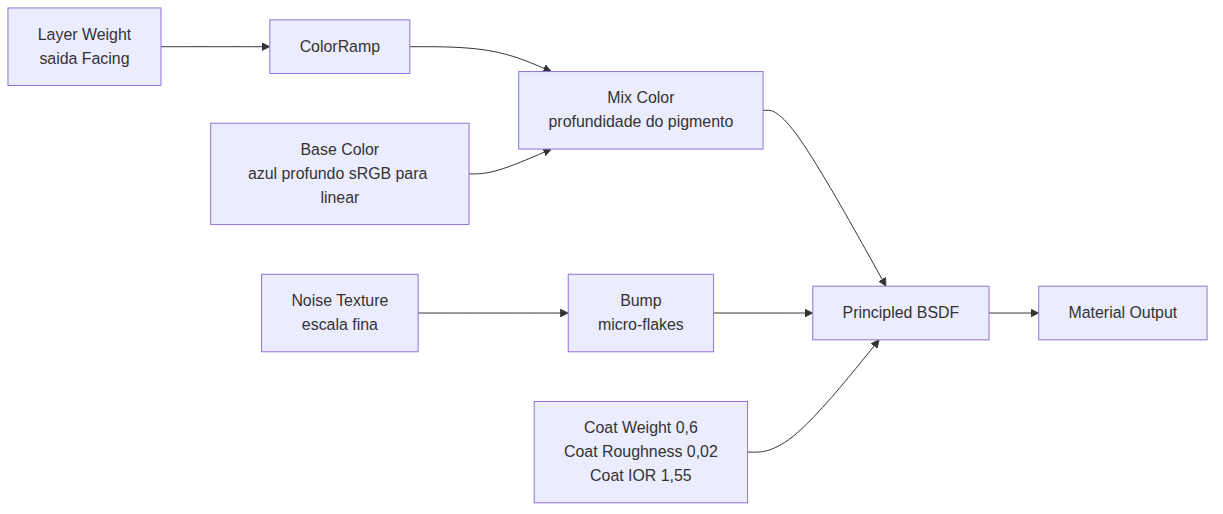
\includegraphics[width=\textwidth]{diagrams/grafo-material-pintura.png}
  \caption{Estrutura do material de pintura. Os tr\^es caminhos --- cor base, micro-relevo e
           verniz --- s\~ao independentes e se combinam no n\'o de sombreamento.}
  \label{fig:material}
  \fonte{elaborado pelo autor (2026).}
\end{figure}

\subsection{Habilita{\c{c}}\~ao da refra{\c{c}}\~ao}

Uma armadilha espec\'ifica do motor EEVEE merece registro. Um material com transmiss\~ao
configurada \emph{n\~ao} refrata automaticamente: \'e necess\'ario habilitar a
refra{\c{c}}\~ao por tra{\c{c}}ado de raios tanto no material quanto na
configura{\c{c}}\~ao de render. O c\'odigo percorre os materiais transparentes e ativa as
propriedades correspondentes, de forma tolerante \`a aus\^encia do atributo em vers\~oes
diferentes:

\begin{lstlisting}[language=Python]
for key in ("glass", "headlamp_lens", "lens_red", "lens_amber"):
    m = mats.get(key)
    if m is None:
        continue
    m.use_screen_refraction = True
    if hasattr(m, "use_raytrace_refraction"):
        m.use_raytrace_refraction = True
    m.blend_method = "BLEND" if hasattr(m, "blend_method") else m.blend_method
\end{lstlisting}

A toler\^ancia por \texttt{hasattr} \'e uma decis\~ao de engenharia defensiva: o script deve
funcionar em vers\~oes pr\'oximas do Blender, degradando de forma controlada em vez de falhar.

\section{O casco principal}\label{sec:casco}

\subsection{Perfil transversal}

O perfil de meio-lado tem nove pontos, definidos em fun{\c{c}}\~ao de sete par\^ametros: a
meia-largura m\'axima $w$, a meia-largura do topo $w_t$, a cota do fundo $z_b$, a cota do ombro
$z_s$, a cota da aresta superior $z_{te}$ e a cota do centro do topo $z_t$. A fun{\c{c}}\~ao
espelha o meio-perfil e fecha o la\c{c}o, resultando em dezesseis pontos por anel.

\begin{lstlisting}[language=Python]
def body_ring(w, wt, zb, zs, zte, zt) -> list[tuple[float, float]]:
    """Half profile mirrored - 16 points, closed loop."""
    span = zs - zb
    zm = zb + 0.58 * span
    half = [
        (0.00, zb),
        (0.40 * w, zb + 0.02 * span),
        (0.80 * w, zb + 0.22 * span),
        (0.97 * w, zb + 0.46 * span),
        (1.00 * w, zm),
        (0.96 * w, zs),
        (0.80 * w, zte - 0.030 * (zt - zte)),
        (0.42 * wt, zte),
        (0.00, zt),
    ]
    return half + [(-y, z) for (y, z) in reversed(half[1:-1])]
\end{lstlisting}

A ordem dos pontos \'e significativa: ela define a dire{\c{c}}\~ao das cadeias de arestas que
percorrem o casco no sentido longitudinal e, portanto, o fluxo de arestas do modelo. Os pontos
4 e 5 concentram a inflex\~ao de largura m\'axima e o ombro, que s\~ao as regi\~oes de maior
curvatura e as que mais influenciam a leitura da silhueta.

\subsection{Esta{\c{c}}\~oes do casco}

O casco \'e definido por \textbf{47 esta{\c{c}}\~oes} transversais, cada uma com sua
s\'extupla $(x, w, w_t, z_s, z_{te}, z_t)$; a cota do fundo \'e calculada, e n\~ao tabelada,
porque depende dos v\~aos de roda. A Tabela~\ref{tab:estacoes-amostra} mostra uma amostra; a
tabela completa est\'a no Ap\^endice~\ref{ap:estacoes}.

\begin{table}[htbp]
\centering
\caption{Amostra de esta{\c{c}}\~oes do casco (valores em metros)}
\label{tab:estacoes-amostra}
\footnotesize
\begin{tabular}{rrrrrr}
\toprule
\textbf{$x$} & \textbf{$w$} & \textbf{$w_t$} & \textbf{$z_s$} & \textbf{$z_{te}$} & \textbf{$z_t$} \\
\midrule
1,863 & 0,625 & 0,500 & 0,470 & 0,560 & 0,592 \\
1,740 & 0,792 & 0,646 & 0,530 & 0,618 & 0,650 \\
1,545 & 0,808 & 0,660 & 0,570 & 0,658 & 0,690 \\
1,150 & 0,820 & 0,660 & 0,680 & 0,742 & 0,766 \\
0,700 & 0,792 & 0,630 & 0,592 & 0,700 & 0,742 \\
0,020 & 0,797 & 0,626 & 0,640 & 0,712 & 0,748 \\
$-0,520$ & 0,832 & 0,648 & 0,692 & 0,812 & 0,872 \\
$-1,150$ & 0,859 & 0,657 & 0,740 & 0,874 & 0,911 \\
$-1,852$ & 0,735 & 0,520 & 0,606 & 0,706 & 0,732 \\
$-1,858$ & 0,735 & 0,520 & 0,606 & 0,706 & 0,732 \\
\bottomrule
\end{tabular}
\fonte{elaborado pelo autor a partir de \texttt{BODY\_STATIONS} (2026).}
\end{table}

Tr\^es caracter\'isticas da tabela merecem leitura. Primeiro, a largura m\'axima ocorre pr\'oximo
ao eixo traseiro ($w = 0,859$\,m em $x = -1,150$), o que reproduz a distribui{\c{c}}\~ao de
massa visual do ve\'iculo real, com a traseira mais larga que a dianteira. Segundo, a cota do
topo cresce de $0,592$\,m no nariz at\'e $0,911$\,m no deck, evidenciando a
inclina{\c{c}}\~ao ascendente da superf\'icie --- a \emph{waistline} referida na
especifica{\c{c}}\~ao. Terceiro, h\'a esta{\c{c}}\~oes repetidas no nariz ($1{,}863$ e
$1{,}856$) e na cauda ($-1{,}852$ e $-1{,}858$): s\~ao an\'eis de reten{\c{c}}\~ao, discutidos
adiante.

O encadeamento \'e feito por uma fun{\c{c}}\~ao que cria os an\'eis e os conecta por quads, com
atribui{\c{c}}\~ao opcional de material por faixa de faces:

\begin{lstlisting}[language=Python]
def build_loft(name, stations, mat_grid=None, cap_mats=(0, 0),
               materials=None, tag_info=None, subsurf=(1, 3),
               smooth=True, caps=True):
    bm = bmesh.new()
    rings = []
    for x, ring in stations:
        rings.append([bm.verts.new((x, y, z)) for (y, z) in ring])
    bm.verts.ensure_lookup_table()
    nseg = len(rings[0])
    bands = []
    for i in range(len(rings) - 1):
        row = []
        for j in range(nseg):
            k = (j + 1) % nseg
            face = bm.faces.new((rings[i][j], rings[i][k],
                                 rings[i + 1][k], rings[i + 1][j]))
            row.append(face)
        bands.append(row)
    if mat_grid is not None:
        for i, row in enumerate(bands):
            for j, face in enumerate(row):
                face.material_index = mat_grid[i][j]
    if caps:
        for end, ring_index in ((0, 0), (1, len(rings) - 1)):
            _folded_fan_cap(bm, list(rings[ring_index]), cap_mats[end], smooth)
    ...
\end{lstlisting}

Como cada face conecta exatamente quatro v\'ertices, a malha resultante \'e quadr\^angular por
constru{\c{c}}\~ao. N\~ao existe etapa de corre{\c{c}}\~ao topol\'ogica posterior: a qualidade
\'e uma propriedade do algoritmo.

\subsection{Arcos de roda sem booleanas}

O recorte do arco \'e obtido por c\'alculo, e n\~ao por subtra{\c{c}}\~ao. Para cada esta{\c{c}}\~ao
$x$, a cota do fundo \'e a maior entre a cota base da carroceria e a circunfer\^encia de cada
arco:

\begin{lstlisting}[language=Python]
def arch_bottom(x, base, arches) -> float:
    """Body bottom accounting for wheel arches."""
    z = base
    for x_axle, z_axle, radius in arches:
        dx = x - x_axle
        if abs(dx) < radius:
            z = max(z, z_axle + math.sqrt(radius * radius - dx * dx))
    return z
\end{lstlisting}

Os par\^ametros s\~ao $(x_{\text{eixo}}, z_{\text{eixo}}, r)$ para cada arco: dianteiro com
raio $0,335$\,m e traseiro com raio $0,350$\,m, ambos centrados na cota do raio do pneu
correspondente. A eleva{\c{c}}\~ao do fundo nas esta{\c{c}}\~oes pr\'oximas ao eixo produz o
``t\'unel'' do arco sem qualquer altera{\c{c}}\~ao na conectividade da malha, o que preserva a
grade quadr\^angular e a continuidade dos reflexos sobre o para-lama.

\subsection{Tampas de extremidade}\label{sec:tampas}

Fechar o nariz e a cauda do \emph{loft} \'e o ponto em que a maioria das implementa{\c{c}}\~oes
ing\^enuas introduz n-gons: o contorno tem dezesseis v\'ertices, e preench\^e-lo com uma \'unica
face produziria um n-gon de dezesseis lados. A biblioteca implementa uma tampa por ``leque
dobrado'', na qual cada quad conecta um par de v\'ertices consecutivos ao par espelhado do lado
oposto do la\c{c}o:

\begin{lstlisting}[language=Python]
def _folded_fan_cap(bm, verts, mat_index, smooth=True):
    """Cap a closed loop using quads only (even n)."""
    n = len(verts)
    if n < 4:
        return []
    if n % 2:
        n -= 1
    created = []
    for i in range(n // 2 - 1):
        a, b = verts[i], verts[i + 1]
        c, d = verts[n - 2 - i], verts[n - 1 - i]
        if len({a, b, c, d}) < 4:
            continue
        try:
            face = bm.faces.new((a, b, c, d))
        except ValueError:
            continue
        face.material_index = mat_index
        created.append(face)
    return created
\end{lstlisting}

A t\'ecnica tem uma consequ\^encia geom\'etrica que precisa ser compreendida: a tampa
resultante n\~ao \'e plana, e sim uma superf\'icie dobrada. Como a regi\~ao \'e
levemente curva e fica nas extremidades do ve\'iculo, o resultado \'e visualmente adequado e,
sobretudo, topologicamente limpo. A alternativa --- aceitar um n-gon e triangular depois ---
seria incompat\'ivel com o requisito de malha.

A mesma fun{\c{c}}\~ao \'e reutilizada para eliminar tampas n-gon geradas pelas primitivas de
cilindro, o que unifica a garantia: qualquer face com mais de quatro lados \'e substitu\'ida por
quads antes de a malha ser convertida em objeto.

\subsection{An\'eis de reten{\c{c}}\~ao}

As esta{\c{c}}\~oes repetidas no nariz e na cauda s\~ao um recurso deliberado. Em subdivis\~ao,
uma sequ\^encia de esta{\c{c}}\~oes muito espa{\c{c}}adas nas extremidades faz com que a
superf\'icie limite retraia e arredonde o contorno --- o resultado \'e o aspecto de
``bal\~ao'' mencionado na an\'alise cr\'itica do projeto. Inserir duas esta{\c{c}}\~oes quase
coincidentes ($1{,}863$ e $1{,}856$; $-1{,}852$ e $-1{,}858$) cria uma
descontinuidade de segunda ordem que ``segura'' o contorno, achatando a face terminal e
estabilizando a silhueta. O custo \'e de tr\^es faces por extremidade --- desprez\'ivel.

\subsection{Rebaixos reais}

Dois recortes s\~ao feitos por deslocamento direto de v\'ertices, com fun{\c{c}}\~ao de
atenua{\c{c}}\~ao suave: as entradas de ar laterais, atr\'as das portas, e o alojamento dos
far\'ois. O primeiro opera apenas nos v\'ertices com $|y| > 0,35$\,m e desloca-os para dentro
segundo uma elipse com profundidade m\'axima de $62$\,mm:

\begin{lstlisting}[language=Python]
def _scoop_dent(obj) -> None:
    """Real side air-intake opening (no boolean, no normal map)."""
    cx, cz = -0.235, 0.520
    rx, rz = 0.215, 0.165
    depth = 0.062
    for v in obj.data.vertices:
        if abs(v.co.y) < 0.35:
            continue
        nx = (v.co.x - cx) / rx
        nz = (v.co.z - cz) / rz
        r = math.sqrt(nx * nx + nz * nz)
        if r >= 1.0:
            continue
        fade = 1.0 if r <= 0.62 else 1.0 - ((r - 0.62) / 0.38) ** 1.5
        sign = 1.0 if v.co.y > 0 else -1.0
        v.co.y -= sign * depth * fade
\end{lstlisting}

O expoente $1,5$ na fun{\c{c}}\~ao de atenua{\c{c}}\~ao foi escolhido para produzir uma
transi{\c{c}}\~ao ligeiramente mais r\'apida que a quadr\'atica, evitando uma borda
excessivamente mole. A profundidade de $62$\,mm supera o m\'inimo de $30$\,mm exigido pelo
requisito FR-006.

O alojamento dos far\'ois usa a mesma estrat\'egia com uma atenua{\c{c}}\~ao c\^onica
suave, escavando $30$\,mm no \emph{clamshell} dianteiro em torno de duas elipses
centradas em $y = \pm0,470$\,m.

\section{Cabine, vidros e interior}\label{sec:cabine}

A cabine \'e um segundo \emph{loft}, assentado sobre a linha de cintura. Seu perfil tem dez
pontos, com topo plano e laterais quase verticais, o que corresponde \`a geometria de um
\emph{hardtop} r\'igido:

\begin{lstlisting}[language=Python]
def cabin_ring(wb, wt, zc, h) -> list[tuple[float, float]]:
    """Cabin profile - flat top, near-vertical sides (10 points)."""
    half = [
        (wb, zc),
        (0.99 * wb, zc + 0.30 * h),
        (0.97 * wb, zc + 0.62 * h),
        (0.90 * wb, zc + 0.88 * h),
        (0.66 * wt, zc + 0.985 * h),
        (0.00, zc + h),
    ]
    return half + [(-y, z) for (y, z) in reversed(half[1:-1])]
\end{lstlisting}

O vidro n\~ao \'e um objeto separado: ele \'e atribu\'ido por \'indice de face, a partir de uma
matriz de material que mapeia cada combina{\c{c}}\~ao de esta{\c{c}}\~ao e segmento do perfil
para um dos dois materiais da cabine. As zonas s\~ao declaradas explicitamente ---
para-brisa, teto, janela traseira e vidros laterais --- e o mapeamento converte a
inten{\c{c}}\~ao de projeto em \'indices:

\begin{lstlisting}[language=Python]
# zones: 0..4 windshield, 5..7 roof, 8..10 rear window, 11+ buttress
windshield = set(range(0, 5))
roof = set(range(5, 8))
rear = {8, 9, 10}
side_glass = {5, 6, 7, 8}
top_segments = {3, 4, 5, 6}
side_segments = {0, 1, 7, 8}
mat_grid = []
for band in range(len(stations) - 1):
    row = []
    for seg in range(10):
        if band in windshield and seg in top_segments:
            row.append(1)
        elif band in rear and seg in top_segments:
            row.append(1)
        elif band in side_glass and seg in side_segments:
            row.append(1)
        else:
            row.append(0)
    mat_grid.append(row)
\end{lstlisting}

A vantagem dessa abordagem \'e que n\~ao existem ``placas'' de vidro flutuando sobre a
carroceria: a superf\'icie do vidro \'e cont\'inua com a do teto, e a transi{\c{c}}\~ao entre
material pintado e vidro ocorre exatamente onde a geometria muda. A desvantagem \'e o
acoplamento entre a defini{\c{c}}\~ao da malha e a defini{\c{c}}\~ao do material: alterar o
n\'umero de esta{\c{c}}\~oes exige revisar as zonas.

O interior \'e simplificado, conforme o escopo: dois assentos (assento e encosto), painel,
volante e santo-ant\'onio, dimensionados para serem lidos atrav\'es dos vidros sem pretender
fidelidade de acabamento interno.

\section{Rodas}\label{sec:rodas}

Cada roda \'e composta por onze objetos: pneu, aro externo, disco do aro, cubo, tampa central,
seis raios, disco de freio e pin{\c{c}}a. O pneu \'e um s\'olido de revolu{\c{c}}\~ao de um perfil
fechado; o aro resulta da revolu{\c{c}}\~ao de um perfil em tr\^es segmentos; e os raios s\~ao
caixas chanfradas posicionadas por rota{\c{c}}\~ao em torno do eixo.

As dimens\~oes v\^em da designa{\c{c}}\~ao comercial dos pneus:

\begin{lstlisting}[language=Python]
TIRE_F_R, RIM_F_R, TIRE_F_HW = 0.292, 0.1905, 0.0925   # 185/55R15
TIRE_R_R, RIM_R_R, TIRE_R_HW = 0.306, 0.2032, 0.1025   # 205/50R16
ARCH_F = (AXLE_F_X, TIRE_F_R, 0.335)
ARCH_R = (AXLE_R_X, TIRE_R_R, 0.350)
\end{lstlisting}

A escolha de derivar o raio do pneu da pr\'opria designa{\c{c}}\~ao --- em vez de estim\'a-lo
da fotografia --- reduz uma fonte de erro: a geometria do pneu \'e conhecida, e o que a
fotografia precisa informar \'e apenas a posi{\c{c}}\~ao relativa do eixo e a altura da
carroceria.

\section{Conjuntos \'opticos}\label{sec:optica}

O farol dianteiro \'e composto por cinco objetos: carca{\c{c}}a, refletor, dois elementos
\'opticos internos e a lente. A carca{\c{c}}a e o refletor s\~ao elipsoides achatados; a lente
\'e uma casca de mesmo contorno, com o material de transmiss\~ao. O conjunto é
assentado dentro do rebaixo escavado no \emph{clamshell}, de modo que a lente fica
aproximadamente no plano da superf\'icie nominal.

A traseira tem quatro lanternas redondas, cada uma com lente e aro met\'alico, mais dois
refletores no difusor. A posi{\c{c}}\~ao das lanternas foi um ponto de corre{\c{c}}\~ao
significativo: como a superf\'icie p\'os-subdivis\~ao recua em rela{\c{c}}\~ao \`a tampa
nominal do \emph{loft}, as lanternas inicialmente ficaram ocultas pela carroceria. A
corre{\c{c}}\~ao consistiu em desloc\'a-las para fora do envelope nominal
($\leq 1,863$\,m), o que exemplifica um modo de falha pr\'oprio de projetos por
subdivis\~ao: a geometria de controle n\~ao \'e a geometria vis\'ivel.

\section{Ventila{\c{c}}\~oes e aerodin\^amica}\label{sec:ventilacoes}

Comp\~oem este grupo a grelha frontal, os \emph{louvers} do \emph{engine cover}, as
sa\'idas de ventila{\c{c}}\~ao traseiras, o difusor, as duas sa\'idas de escape centrais, o
\emph{splitter} dianteiro e as aletas do difusor. A grelha frontal \'e um painel
rebaixado com cinco aletas; os \emph{louvers} s\~ao doze l\^aminas
distribu\'idas em duas fileiras, cada uma uma caixa chanfrada inclinada.

Uma decis\~ao de corre{\c{c}}\~ao merece registro: a grelha e as inser{\c{c}}\~oes
\'opticas s\~ao objetos \emph{assentados} sobre a superf\'icie, e n\~ao recortes perfurados. A
raz\~ao \'e geom\'etrica: a tampa do \emph{loft} n\~ao possui v\'ertices internos que
permitam escavar uma abertura sem recorrer a uma opera{\c{c}}\~ao booleana --- que o requisito
pro\'ibe. Essa escolha \'e registrada como desvio de especifica{\c{c}}\~ao, e n\~ao como
atendimento pleno do requisito.

\section{Emblemas}\label{sec:emblemas}

Os emblemas \texttt{LOTUS} e \texttt{111S} s\~ao textos tridimensionais convertidos em malha. O
processo cria um objeto de texto, define corpo, tamanho, extrus\~ao, alinhamento e
espa{\c{c}}amento entre caracteres, e converte a curva resultante em malha. O par\^ametro de
espa{\c{c}}amento foi necess\'ario porque o \emph{tracking} padr\~ao da fonte deixava os
caracteres excessivamente separados em rela{\c{c}}\~ao \`a refer\^encia.

\begin{lstlisting}[language=Python]
def text_mesh(name, body, size, extrude, location=(0, 0, 0),
              rotation=(0, 0, 0), material=None, tag_info=None,
              align_x="CENTER", align_y="CENTER", spacing=1.0):
    curve = bpy.data.curves.new(name=name, type="FONT")
    curve.body = body
    curve.size = size
    curve.extrude = extrude
    curve.align_x = align_x
    curve.align_y = align_y
    curve.space_character = spacing
    obj = bpy.data.objects.new(name, curve)
    bpy.context.scene.collection.objects.link(obj)
    bpy.context.view_layer.objects.active = obj
    bpy.ops.object.convert(target="MESH")
    ...
\end{lstlisting}

Os glifos t\^em contorno aberto, o que gera arestas de borda na malha resultante. Essas arestas
n\~ao s\~ao n\~ao variedade --- portanto n\~ao violam o requisito --- mas s\~ao a
\emph{\'unica} origem das 1.776 arestas de borda registradas no relat\'orio. A
corre{\c{c}}\~ao indicada \'e substituir o texto por glifos de contorno fechado, extrusados; a
solu{\c{c}}\~ao n\~ao foi aplicada nesta vers\~ao e est\'a registrada como pend\^encia.

\section{Nomenclatura, metadados e subdivis\~ao}\label{sec:nomenclatura}

Todo objeto recebe um prefixo de categoria: \texttt{GEO\_} para geometria, \texttt{LGT\_} para
luzes e \texttt{CAM\_} para c\^ameras. Al\'em do nome, cada objeto de geometria recebe tr\^es
propriedades personalizadas, gravadas pela fun{\c{c}}\~ao \texttt{tag}:

\begin{lstlisting}[language=Python]
def tag(obj, cat: str, part: str, swap: str) -> None:
    """Metadata for automated material swap via MCP."""
    obj["cat"] = cat
    obj["part"] = part
    obj["mat_swap_key"] = swap
\end{lstlisting}

O objetivo declarado \'e permitir troca automatizada de material: um agente pode localizar
todos os objetos cujo \texttt{mat\_swap\_key} seja \texttt{paint\_primary} e substituir o
material sem inspecionar nomes de objeto. \'E um exemplo de como a conven{\c{c}}\~ao de
nomenclatura deixa de ser est\'etica e passa a ser uma interface de programa{\c{c}}\~ao.

Os dois corpos principais recebem o modificador de subdivis\~ao com n\'ivel de
visualiza{\c{c}}\~ao 1 e n\'ivel de render 3. A assimetria \'e deliberada: o n\'ivel 3 no
render garante a suavidade do resultado final, enquanto o n\'ivel 1 na
visualiza{\c{c}}\~ao mant\'em a resposta da interface utiliz\'avel --- requisito pr\'atico
para quem precisa inspecionar a cena.

\section{Relat\'orio de malha}\label{sec:relatorio-malha}

O \emph{build} termina emitindo um relat\'orio em formato de texto, com uma linha por objeto e
totais consolidados. O relat\'orio \'e a evid\^encia prim\'aria de integridade estrutural, e
cont\'em: contagem de v\'ertices, faces, quads, tri\^angulos e n-gons por objeto; arestas
n\~ao variedade; arestas de borda; e o envelope dimensional com a diferen{\c{c}}a em
rela{\c{c}}\~ao aos alvos.

O envelope \'e calculado varrendo os oito cantos da caixa delimitadora de cada objeto de malha,
transformados para coordenadas de mundo:

\begin{lstlisting}[language=Python]
def world_bounds(objects=None) -> dict:
    objs = objects if objects is not None else bpy.data.objects
    lo = Vector((1e9, 1e9, 1e9))
    hi = Vector((-1e9, -1e9, -1e9))
    for obj in objs:
        if obj.type != "MESH":
            continue
        for corner in obj.bound_box:
            p = obj.matrix_world @ Vector(corner)
            lo = Vector((min(lo.x, p.x), min(lo.y, p.y), min(lo.z, p.z)))
            hi = Vector((max(hi.x, p.x), max(hi.y, p.y), max(hi.z, p.z)))
    return dict(min=lo, max=hi, size=hi - lo)
\end{lstlisting}

A escolha de medir a caixa delimitadora dos objetos, e n\~ao os v\'ertices da malha de
controle, \'e relevante: \'e a geometria avaliada que define o envelope percebido. O
relat\'orio \'e gravado em \texttt{docs/renders/mesh\_report.txt} e reproduzido no
Ap\^endice~\ref{ap:objetos}.

\section{Rig de verifica{\c{c}}\~ao e c\^ameras}

O rig de verifica{\c{c}}\~ao tem quatro luzes de \'area retangulares: uma chave, um
preenchimento, uma luz de recorte e um cart\~ao longo lateral. As quatro s\~ao
direcionadas para um ponto comum por uma fun{\c{c}}\~ao auxiliar que converte a
dire{\c{c}}\~ao em rota{\c{c}}\~ao de rastreamento:

\begin{lstlisting}[language=Python]
def _aim(obj, target=(0.0, 0.0, 0.55)) -> None:
    direction = Vector(target) - obj.location
    obj.rotation_euler = direction.to_track_quat("-Z", "Y").to_euler()
\end{lstlisting}

As nove c\^ameras formam um conjunto de verifica{\c{c}}\~ao e de apresenta{\c{c}}\~ao. A
Quadro~\ref{qua:cameras} lista as c\^ameras com dist\^ancia focal e posi{\c{c}}\~ao. A
vista superior usa rota{\c{c}}\~ao expl\'icita em vez de rastreamento, porque o rastreamento
com alvo diretamente abaixo produz uma rota{\c{c}}\~ao degenerada.

\begin{quadro}[htbp]
\centering
\caption{C\^ameras do conjunto e par\^ametros principais}
\label{qua:cameras}
\footnotesize
\begin{tabular}{>{\raggedright\arraybackslash}p{3.6cm}>{\raggedright\arraybackslash}p{3.4cm}>{\raggedright\arraybackslash}p{1.7cm}>{\raggedright\arraybackslash}p{3.9cm}}
\toprule
\textbf{C\^amera} & \textbf{Posi{\c{c}}\~ao (m)} & \textbf{Focal} & \textbf{Papel} \\
\midrule
\texttt{CAM\_Frontal} & (7,6; 0; 0,72) & 95 mm & vista frontal \\
\texttt{CAM\_Lateral} & (0; 8,2; 0,76) & 62 mm & vista lateral \\
\texttt{CAM\_Traseira} & ($-$7,6; 0; 0,78) & 95 mm & vista traseira \\
\texttt{CAM\_Superior} & (0; 0; 10,5) & 50 mm & vista superior \\
\texttt{CAM\_WheelDetail} & (2,05; 1,35; 0,50) & 78 mm & detalhe de roda \\
\texttt{CAM\_TresQuartos} & (4,95; 4,15; 1,95) & 72 mm & tr\^es-quartos \\
\texttt{CAM\_TresQuartos\_Tr} & ($-$4,95; 4,15; 1,95) & 72 mm & tr\^es-quartos traseiro \\
\texttt{CAM\_Isometrica} & (5,40; 5,40; 3,90) & 70 mm & isom\'etrica \\
\texttt{CAM\_Hero} & (4,90; 3,80; 1,00) & 50 mm & apresenta{\c{c}}\~ao \\
\bottomrule
\end{tabular}
\fonte{elaborado pelo autor a partir de \texttt{build\_cameras} (2026).}
\end{quadro}

\section{Configura{\c{c}}\~ao de render e mudan{\c{c}}as de API}\label{sec:api-blender}

A configura{\c{c}}\~ao de render \'e feita por c\'odigo e precisa acomodar mudan{\c{c}}as
introduzidas nas vers\~oes recentes do Blender. Tr\^es delas afetam diretamente este projeto e
s\~ao tratadas defensivamente.

\textbf{Aus\^encia do \'arvore de composi{\c{c}}\~ao na cena.} Nas vers\~oes anteriores, o
compositor era acessado por uma propriedade da cena. Na vers\~ao utilizada, o compositor \'e um
grupo de n\'os criado separadamente e associado \`a cena, e o n\'o de sa\'ida
\texttt{Composite} foi substitu\'ido por um n\'o de sa\'ida de grupo.

\textbf{Aus\^encia do efeito de brilho no motor.} O par\^ametro de \emph{bloom} deixou de
existir; o brilho passou a ser obtido por um n\'o de \emph{glare} no compositor, com tipo,
limiar, tamanho e intensidade configurados como entradas do n\'o.

\textbf{Nomes de opera{\c{c}}\~oes de cor.} Os nomes v\'alidos do \emph{look} de
mapeamento de tons variam entre vers\~oes, e um nome inv\'alido interrompe a
execu{\c{c}}\~ao. A solu{\c{c}}\~ao adotada \'e uma tentativa em cascata:

\begin{lstlisting}[language=Python]
scene.view_settings.view_transform = "AgX"
for look in ("AgX - Medium High Contrast", "AgX - Base Contrast", "None"):
    try:
        scene.view_settings.look = look
        break
    except Exception:
        continue
scene.view_settings.exposure = -0.18
for attr, value in (("taa_render_samples", 96),
                    ("use_raytracing", True),
                    ("use_shadows", True)):
    if hasattr(scene.eevee, attr):
        try:
            setattr(scene.eevee, attr, value)
        except Exception:
            pass
\end{lstlisting}

O padr\~ao \'e sempre o mesmo: verificar a exist\^encia do atributo antes de us\'a-lo, e
falhar de forma tolerante. Em um contexto de automa{\c{c}}\~ao por agente, essa disciplina tem
valor adicional: uma exce{\c{c}}\~ao n\~ao tratada interrompe a sess\~ao e obriga a um novo ciclo
de diagn\'ostico, enquanto uma degrada{\c{c}}\~ao controlada mant\'em o pipeline
execut\'avel.

Uma armadilha adicional, de natureza diferente, foi verificada: a atribui{\c{c}}\~ao de escala a
um objeto exige uma tupla de tr\^es elementos. Constru{\c{c}}\~oes que produzem tuplas de tamanho
vari\'avel --- como a repeti{\c{c}}\~ao de um valor --- n\~ao s\~ao aceitas nessa
atribui{\c{c}}\~ao. \'E um exemplo de erro que s\'o se manifesta em tempo de execu{\c{c}}\~ao
dentro do Blender, e que refor{\c{c}}a a necessidade de valida{\c{c}}\~ao sint\'atica
pr\'evia do c\'odigo gerado.

\section{A galeria de apresenta{\c{c}}\~ao}\label{sec:galeria}

A galeria produz cinco imagens: superior, traseira, lateral, isom\'etrica e uma imagem com
efeito de luz. As quatro primeiras usam o rig neutro. A quinta usa um rig dram\'atico
tempor\'ario, com luzes de recorte laterais, emiss\~ao nos elementos \'opticos dianteiros e
brilho no compositor. Ao final, o script restaura o rig neutro e \emph{n\~ao} grava o arquivo
de cena.

A decis\~ao de n\~ao persistir o rig dram\'atico \'e deliberada: ele \'e um artefato de
apresenta{\c{c}}\~ao, e n\~ao um estado do modelo. Persisti-lo contaminaria o ambiente de
verifica{\c{c}}\~ao e quebraria a reprodutibilidade dos renders neutros. A
Figura~\ref{fig:galeria-luz} mostra o resultado do rig dram\'atico.

\begin{figure}[htbp]
  \centering
  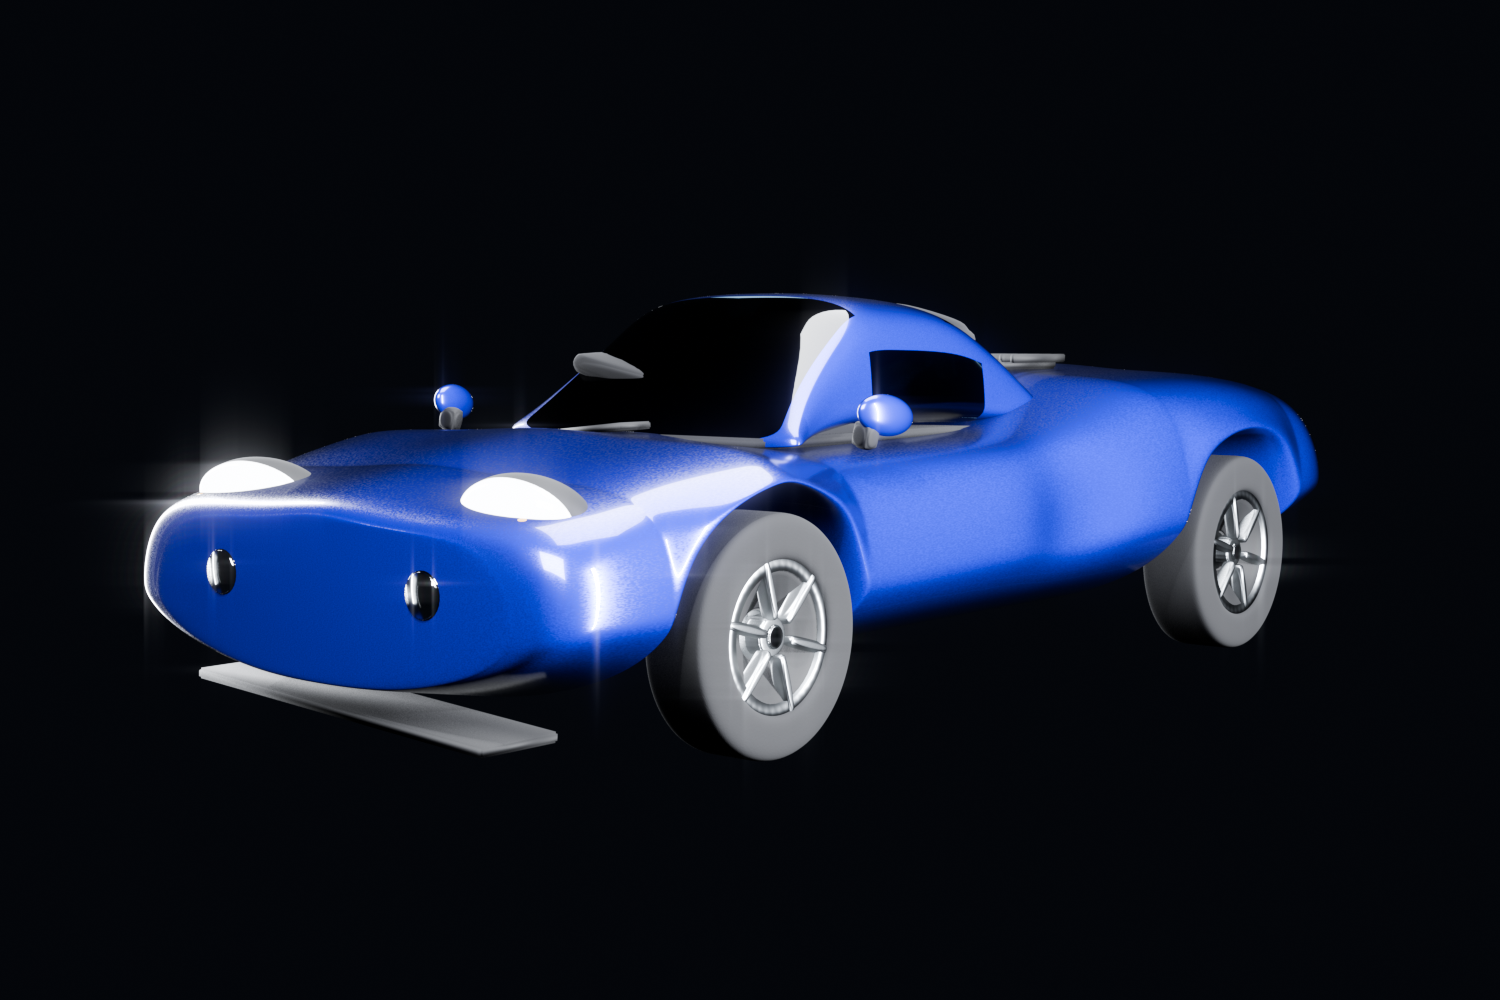
\includegraphics[width=0.92\textwidth]{figures/gal-luz.png}
  \caption{Imagem de apresenta{\c{c}}\~ao com rig dram\'atico tempor\'ario: luzes de recorte
           laterais, elementos \'opticos acesos e brilho via n\'o de \emph{glare}.}
  \label{fig:galeria-luz}
  \fonte{elaborado pelo autor (2026).}
\end{figure}

\section{O ciclo de chamadas via MCP}\label{sec:mcp-ciclo}

A opera{\c{c}}\~ao por MCP reduz o ciclo de trabalho a tr\^es ferramentas: executar c\'odigo,
consultar a cena e capturar a imagem da \emph{viewport}. O ciclo completo de uma
itera{\c{c}}\~ao \'e apresentado na Figura~\ref{fig:sequencia}.

\begin{figure}[htbp]
  \centering
  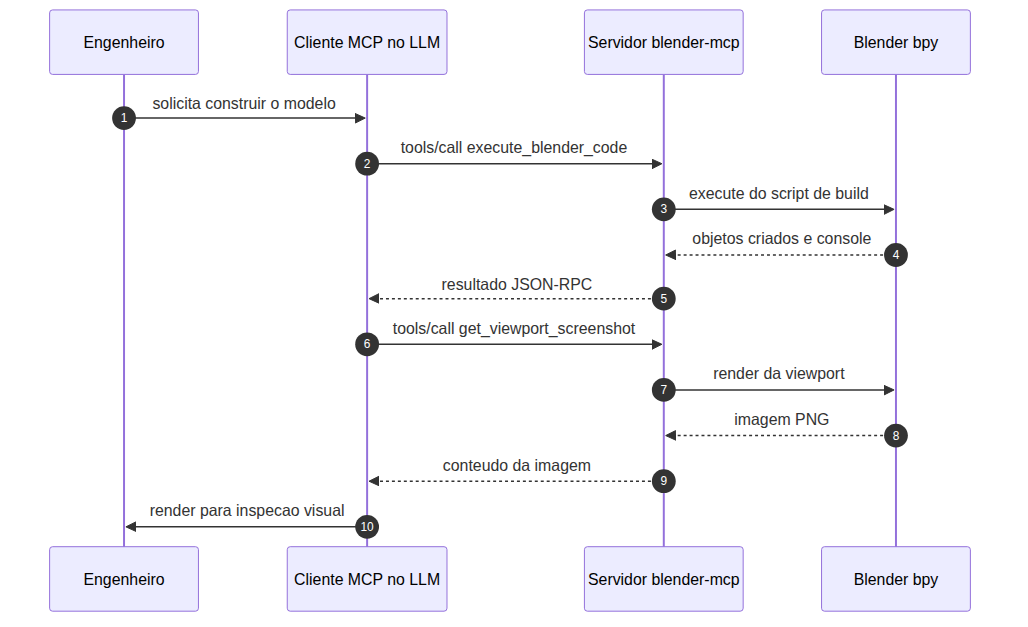
\includegraphics[width=\textwidth]{diagrams/sequencia-build.png}
  \caption{Ciclo de chamadas do protocolo durante um ciclo de constru{\c{c}}\~ao e
           inspe{\c{c}}\~ao. Cada chamada \'e uma mensagem serializada, o que constitui o
           registro audit\'avel do processo.}
  \label{fig:sequencia}
  \fonte{elaborado pelo autor (2026).}
\end{figure}

O encadeamento tem uma propriedade importante: a mensagem de execu{\c{c}}\~ao \'e, ela
pr\'opria, o artefato de reprodutibilidade. Executar o mesmo script por linha de comando ou
por MCP produz a mesma cena, porque nos dois casos o que se executa \'e o mesmo c\'odigo. A
diferen{\c{c}}a entre os dois modos est\'a no \emph{registro}: no modo MCP, os argumentos e
resultados ficam serializados; no modo linha de comando, restam no hist\'orico do terminal.

Uma limita{\c{c}}\~ao merece ser dita com clareza. A inspe{\c{c}}\~ao visual mediada por MCP
consiste em uma captura bidimensional. A avalia{\c{c}}\~ao de continuidade de superf\'icie por
essa via \'e inferior \`a inspe{\c{c}}\~ao interativa, na qual o avaliador pode orbitar a cena e
observar o comportamento especular sob movimento. O presente trabalho compensa essa
limita{\c{c}}\~ao com duas provid\^encias: a captura de vistas m\'ultiplas predefinidas e a
verifica{\c{c}}\~ao num\'erica das propriedades estruturais. Ainda assim, a limita{\c{c}}\~ao
permanece e \'e registrada como tal.
